\documentclass[10pt]{article}
\usepackage{amsmath,amsthm,amssymb,dsfont,graphicx,xspace,epsfig,xcolor}
\usepackage{tikz, tkz-graph, tkz-berge}
\usetikzlibrary{decorations.pathreplacing}
\usetikzlibrary{patterns}
\usetikzlibrary{patterns.meta}
\usepackage{color}

\begin{document}

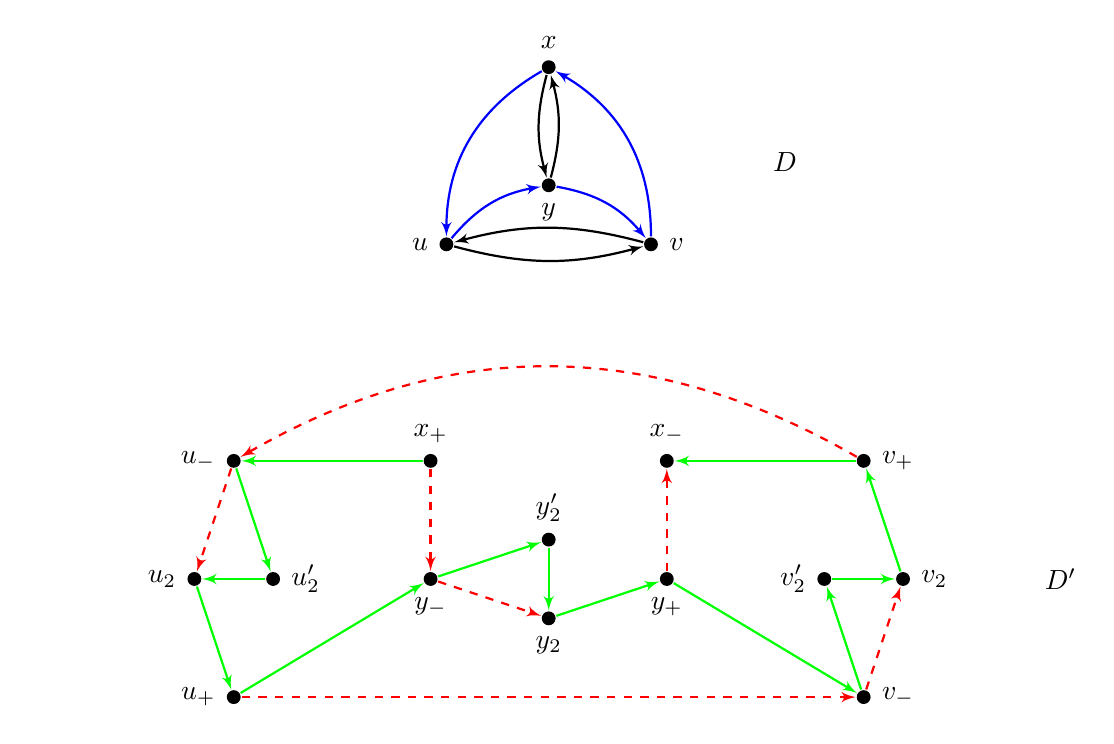
\begin{tikzpicture}[thick,scale=1, every node/.style={transform shape}]
      \tikzset{vertex/.style = {circle,fill=black,minimum size=5pt, inner sep=0pt}}
      \tikzset{edge/.style = {->,> = latex'}}

      \node[vertex,label=above:$x$] (x) at (90:1.5){};
      \node[vertex,label=below:$y$] (y) at (0,0){};
      \node[vertex,label=left:$u$] (u) at (210:1.5){};
      \node[vertex,label=right:$v$] (v) at (-30:1.5){};
      \draw[edge,blue] (x) to[out=-150, in=90] (u){};
      \draw[edge,blue] (u) to[out=50, in=-170] (y){};
      \draw[edge,blue] (y) to[out=-10, in=130] (v){};
      \draw[edge,blue] (v) to[out=90, in=-30] (x){};
      \draw[edge, bend right=15] (x) to (y){};
      \draw[edge, bend right=15] (y) to (x){};
      \draw[edge, bend right=15] (v) to (u){};
      \draw[edge, bend right=15] (u) to (v){};
      \node[] (D) at (3,0.3) {$D$};

      \begin{scope}[yshift=-5cm]
      \node[vertex,label=above:$x_-$] (xm) at (1.5,1.5){};
      \node[vertex,label=above:$x_+$] (xp) at (-1.5,1.5){};

      \node[vertex,label=below:$y_-$] (ym) at (-1.5,0){};
      \node[vertex,label=below:$y_+$] (yp) at (1.5,0) {};
      \node[vertex,label=below:$y_2$] (y2) at (0,-0.5){};
      \node[vertex,label=above:$y_2'$] (y22) at (0,0.5){};

      \node[vertex,label=left:$u_-$] (um) at (-4,1.5){};
      \node[vertex,label=left:$u_+$] (up) at (-4,-1.5) {};
      \node[vertex,label=left:$u_2$] (u2) at (-4.5,0){};
      \node[vertex,label=right:$u_2'$] (u22) at (-3.5,0){};

      \node[vertex,label=right:$v_-$] (vm) at (4,-1.5){};
      \node[vertex,label=right:$v_+$] (vp) at (4,1.5) {};
      \node[vertex,label=right:$v_2$] (v2) at (4.5,0){};
      \node[vertex,label=left:$v_2'$] (v22) at (3.5,0){};

      \draw[edge,green] (xp) to (um){};
      \draw[edge,green] (up) to (ym){};
      \draw[edge,green] (yp) to (vm){};
      \draw[edge,green] (vp) to (xm){};
      \draw[edge,red, dashed] (xp) to (ym){};
      \draw[edge,red, dashed] (yp) to (xm){};
      \draw[edge,red, dashed] (vp) to[out=150, in=30] (um){};
      \draw[edge,red, dashed] (up) to (vm){};

      \draw[edge,green] (ym) to (y22){};
      \draw[edge, red, dashed] (ym) to (y2){};
      \draw[edge,green] (y22) to (y2){};
      \draw[edge,green] (y2) to (yp){};

      \draw[edge,green] (um) to (u22){};
      \draw[edge, red, dashed] (um) to (u2){};
      \draw[edge,green] (u22) to (u2){};
      \draw[edge,green] (u2) to (up){};

      \draw[edge,green] (vm) to (v22){};
      \draw[edge, red, dashed] (vm) to (v2){};
      \draw[edge,green] (v22) to (v2){};
      \draw[edge,green] (v2) to (vp){};

      \node[] (Dp) at (6.5,0) {$D'$};
      \node[] (Dp2) at (-6.5,0) {};
      \end{scope}

  \end{tikzpicture}

\end{document}